\section{Lenguajes nativos}

\begin{frame}[t]{Programa nativo}
  \begin{itemize}
    \item Un \textbf{programa nativo} es un programa de computador que se ejecuta directamente en el juego de instrucciones de la máquina.
      \begin{itemize}
        \item Contiene instrucciones de la ISA sobre la que se ejecuta.
        \item No requiere ninguna traducción durante su ejecución.
        \item Puede contener llamadas a un sistema operativo concreto.
      \end{itemize}
  \end{itemize}
\end{frame}

\begin{frame}[t]{Ensamblador}
  \begin{itemize}
    \item Decada de los 40:
      \begin{itemize}
        \item Programas en código máquina codificados directamente comos secuencia de valores binarios.
        \item Aparece la idea de ensamblador.
      \end{itemize}
  \end{itemize}

\begin{columns}
  \begin{column}{0.2\textwidth}
    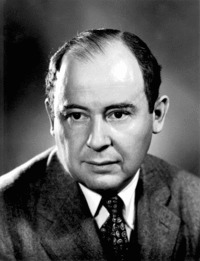
\includegraphics[width=.8\textwidth]{images/von-neumann.jpg}
  \end{column}
  \begin{column}{0.8\textwidth}
    \begin{quote}
      Why would you want more than machine language?
    \end{quote}
    John von Neumann (1903-1957)
  \end{column}
\end{columns}

\begin{itemize}
  \item Aparecen lenguajes ensambladores y herramientas asociadas:
    \begin{itemize}
      \item Ensamblador (assembler): Traduce a código objeto.
      \item Editro de enlaces (linker): Fusiona módulos de código objeto en un ejecutable en código máquina.
    \end{itemize}
\end{itemize}
\end{frame}

\begin{frame}[t]{Problemas con el ensamblador}
\end{frame}

\begin{frame}[t]{Lenguajes de programación}
\end{frame}

